% Sophism density per goal across substrates (the headline discriminative axis).
% Uses pgfplots. Designed for full text-width or single column.
\begin{figure}[t]
\centering
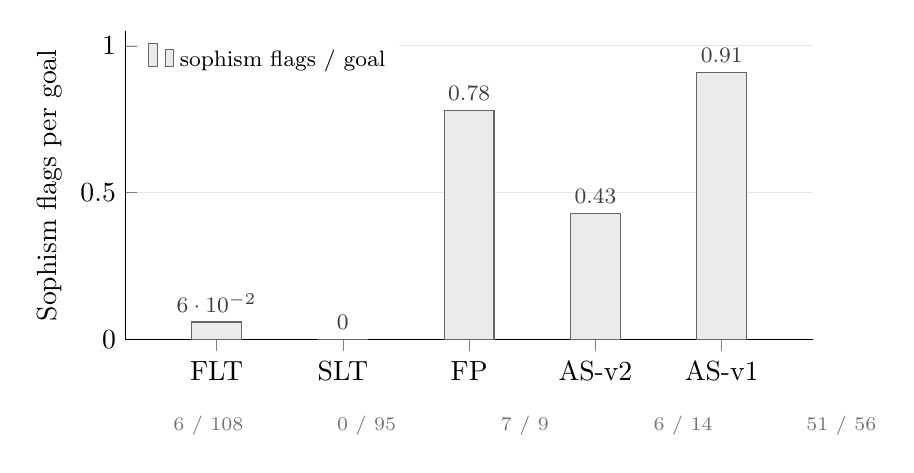
\begin{tikzpicture}
\begin{axis}[
  width=0.85\textwidth,
  height=5.5cm,
  ybar,
  bar width=18pt,
  enlarge x limits=0.18,
  ymin=0,
  ymax=1.05,
  ylabel={Sophism flags per goal},
  xlabel={},
  symbolic x coords={FLT, SLT, FP, AS-v2, AS-v1},
  xtick=data,
  nodes near coords,
  nodes near coords style={font=\footnotesize},
  ymajorgrids,
  major grid style={black!10},
  axis lines*=left,
  tick style={black!50},
  every node near coord/.append style={font=\footnotesize, color=black!75},
  legend style={
    at={(0.02,0.98)},
    anchor=north west,
    draw=none,
    fill=white,
    font=\footnotesize,
  },
]
\addplot[fill=black!8, draw=black!60] coordinates {
  (FLT, 0.06)
  (SLT, 0.00)
  (FP, 0.78)
  (AS-v2, 0.43)
  (AS-v1, 0.91)
};
\addlegendentry{sophism flags / goal}

\end{axis}

% Absolute-count annotations below the x-axis labels (in tikzpicture coords).
\node[font=\scriptsize, anchor=north, black!55] at (1.05, -0.85) {6 / 108};
\node[font=\scriptsize, anchor=north, black!55] at (3.06, -0.85) {0 / 95};
\node[font=\scriptsize, anchor=north, black!55] at (5.07, -0.85) {7 / 9};
\node[font=\scriptsize, anchor=north, black!55] at (7.08, -0.85) {6 / 14};
\node[font=\scriptsize, anchor=north, black!55] at (9.09, -0.85) {51 / 56};
\end{tikzpicture}
\caption{Sophism flag density across the five substrates. The two
pre-verified-clean Lean substrates (FLT, SLT) sit near zero. The two
autonomous-AI-generated paper substrates (AS-v1, AS-v2) and the public
mathematical research benchmark (FP) sit substantially higher. Counts shown
below each bar are flagged records over total goal records.
The discriminative gap (Lean substrates: 6 sophism flags over 203 goals,
0.03/goal; AS papers: 57 over 70, 0.81/goal) is approximately 27$\times$ ---
the rubric resolves the substrates that the headline accept/reject metric
cannot.}
\label{fig:sophism_density}
\end{figure}
